\documentclass[5p,final]{elsarticle}

% Text
% \usepackage{textcomp} % Reinsert if not loading stix2
\usepackage[T1]{fontenc}

% Math, CS, graphics
\usepackage{amsmath,amssymb,graphicx}
\usepackage{algorithm}
\usepackage[indLines=false]{algpseudocodex}
\usepackage{texlogos}
\usepackage{tikz}
\usetikzlibrary{arrows.meta, patterns, positioning, shapes.arrows,
decorations.pathreplacing}

% Miscellaneous formatting
\usepackage[autostyle=true,style=american]{csquotes}
\usepackage[activate={true,nocompatibility}, final, tracking=true,
kerning=true, spacing=true]{microtype}
\usepackage[strings]{underscore}
\usepackage{xurl}
\microtypecontext{spacing=nonfrench}

% Bibliography
\usepackage{listingsutf8}

% Layout
\usepackage{adjustbox}
\usepackage{float}

% els-dc formatting
\RequirePackage{etoolbox,balance}
\RequirePackage{booktabs,makecell,multirow,array,colortbl,dcolumn,stfloats}
\RequirePackage{xspace,xstring,footmisc}
\biboptions{numbers,sort&compress}
\RequirePackage{stix2}
\RequirePackage{CharisSIL} % I would expect Gulliver, but this is very similar
\usepackage[svgnames,dvipsnames]{xcolor}
\RequirePackage{booktabs,makecell,multirow,array,colortbl,dcolumn,stfloats}
\RequirePackage[colorlinks]{hyperref}
\AtBeginDocument{%
	\hypersetup{%
		pdftitle={\csuse{__short_title:}},
		pdfauthor={\csuse{__short_authors:}},
		linkcolor={DarkSlateGray},
		urlcolor={DarkSlateGray},
		citecolor={DarkSlateGray},
		filecolor={DarkSlateGray},
menucolor={DarkSlateGray}}}
\usepackage[hypcap=true]{caption}
\usepackage[hypcap=true]{subcaption}

% ORCID
\usepackage{orcidlink}

\newcommand{\plotspath}{paper-dependencies/latex-dependencies/plots}
\newcommand{\supplementalsurl}{\url{https://github.com/mitre/fast-search-for-tlsh}}
\newcommand{\tlshhash}{ABCDEF\ldots}

\journal{Forensic Science International: Digital Investigation}

\begin{document}
\begin{frontmatter}
	\title{If At First You Don't Succeed, Trie, Trie Again: Correcting
	TLSH Scalability Claims for Large-Dataset Malware Forensics}

	\author[mitre]{Jordi Gonzalez\,\orcidlink{0009-0000-8585-9575}\,\corref{cor1}}
	\ead{jgonzalez@mitre.org}

	\affiliation[mitre]{organization={The MITRE Corporation},
		addressline={7525 Colshire Drive},
		city={McLean},
		postcode={22102},
		state={VA},
	country={USA}}

	\cortext[cor1]{Corresponding author}

	\begin{abstract}
		Malware analysts use Trend Micro Locality-Sensitive Hashing (TLSH)
		for malware similarity computation, nearest-neighbor search, and
		related tasks like clustering and family classification. Although
		TLSH scales better than many alternatives, technical limitations
		have limited its application to larger datasets. Using the Lean 4
		proof assistant, I formalized bounds on the properties of TLSH most
		relevant to its scalability and identified flaws in prior TLSH
		nearest-neighbor search algorithms. I leveraged these formal
		results to design correct acceleration structures for TLSH
		nearest-neighbor queries. On typical analyst workloads, these
		structures performed one to two orders of magnitude faster than the
		prior state-of-the-art, allowing analysts to use datasets at least
		an order of magnitude larger than what was previously feasible with
		the same computational resources. I make all code and data publicly available.
	\end{abstract}

	\begin{keyword}
		Locality-sensitive hashing \sep Malware analysis
	\end{keyword}
\end{frontmatter}

\section{Introduction}

The growing volume of both malicious and benign software presents a
growing burden to malware analysts and security vendors. They must
accurately identify connections between malware samples while
avoiding false associations between innocuous files and
malware, and between unrelated malware families.

Locality-sensitive hashing (LSH)
\cite{indykApproximateNearestNeighbors1998,haqSurveyBinaryCode2021}
helps analysts solve this problem by providing a precise
\cite{oliverTLSHLocalitySensitive2013} dimensionality
reduction technique, whereby more similar pieces of software have
higher spatial proximity. This capability enables at-scale
nearest-neighbor searches and, in turn, clustering
\cite{oliverFastClusteringHigh2021, bakClusteringIoTMalware2020},
antivirus whitelisting \cite{SmartWhitelistingUsing2017},
detection
\cite{intelligenceCombingFuzzUsing2021,naikRansomwareDetectionMethod2019},
malware campaign tracking \cite{naikCyberthreatHuntingPart2019}, and
confidentiality-preserving threat information sharing
\cite{almahmoudHashCombHierarchicalDistancePreserving2022}.

Trend Micro Locality-Sensitive Hashing
\cite{oliverTLSHLocalitySensitive2013,oliverGitHubTrendmicroTlsh2024} (TLSH)
emerged as a standard locality-sensitive hash function for
malware analysis. However, efficiently searching for similar hashes
in large TLSH datasets remains a challenge: even though it is possible
to compute TLSH hashes rapidly for a set of inputs, and even though
it is possible to compare different pairs of hashes rapidly, finding
nearest-neighbors is computationally demanding and scales poorly with
corpora size. The root of this issue is in the TLSH distance
function, which violates the triangle inequality and, therefore,
limits the use of metric data structures for nearest-neighbor
searches. No correct, non-approximate, publicly available algorithm
was found that addressed this gap. This work makes several contributions
toward closing it.

First, this work uses the Lean 4 theorem prover
\cite{deMouraUllrich2021} to provide formal, tight bounds on the triangle
inequality violations for the TLSH distance function and its various
subcomponents. This exposes an error in prior research that underestimated the
bounds by a factor of over 20 (see \autoref{tab:tlsh_violations}).

Second, based on those theoretical results, this work presents two
TLSH-specific nearest-neighbor acceleration structures: one, based on
tries \cite{fredkinTrieMemory1960}, and another, based on
vantage-point (VP) trees
\cite{yianilosDataStructuresAlgorithms1993,uhlmannSatisfyingGeneralProximity1991}.

Third, this work evaluates the performance of these structures on real-world
and synthetic data, demonstrating >10x throughput on common workloads compared
to corrected versions of the prior state-of-the-art.

Finally, all code is made available at \supplementalsurl.

\section{Background}

\subsection{Design of TLSH}

The TLSH whitepaper \cite{oliverTLSHLocalitySensitive2013} accurately
describes TLSH behavior. This subsection summarizes the aspects of
the whitepaper most relevant to this work.

TLSH maps arbitrary byte streams to fixed-length hashes. The hashes
are split into a \enquote{header} component and a \enquote{body}
component. As illustrated in \autoref{fig:tlsh_structure}, these
two components have several subcomponents, or \enquote{features.}
The precise semantics of these features are unimportant to this
work, but their layout is illustrated by \autoref{fig:tlsh_structure}.

\begin{figure}[H]
	\centering
	\begin{adjustbox}{width=\columnwidth}
		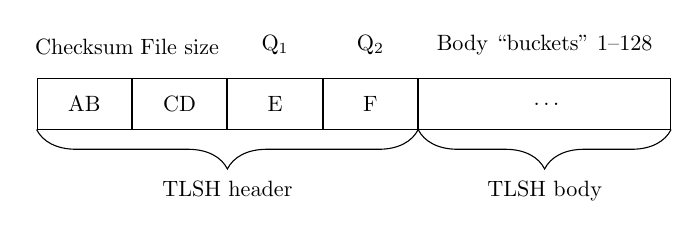
\begin{tikzpicture}[
				every node/.style={align=center},
				component/.style={draw, rectangle, minimum height=.8cm, minimum
				width=1.5cm, anchor=west},
				scale=0.8,
				transform shape
			]

			\node[component] (checksum) at (0,0) {\StrMid{\tlshhash}{1}{2}};
			\node[component, right=0cm of checksum] (lvalue) {\StrMid{\tlshhash}{3}{4}};
			\node[component, right=0cm of lvalue] (q1value) {\StrMid{\tlshhash}{5}{5}};
			\node[component, right=0cm of q1value] (q2value) {\StrMid{\tlshhash}{6}{6}};
			\node[component, right=0cm of q2value, minimum width=4cm] (body)
			{\StrMid{\tlshhash}{7}{70}};

			\node[above=0.25cm of checksum] (label1) {Checksum};
			\node[above=0.25cm of lvalue] (label2) {File size};	
			\node[above=0.25cm of q1value] (label3) {Q\textsubscript{1}};	
			\node[above=0.25cm of q2value] (label4) {Q\textsubscript{2}};
			\node[above=0.25cm of body] (label5) {Body \enquote{buckets} 1--128};

			\draw[decorate,decoration={brace,amplitude=.5cm,mirror}]
			(checksum.south west) -- (q2value.south east)
			node[midway,below=.7cm] {TLSH header};

			\draw[decorate,decoration={brace,amplitude=.5cm,mirror}]
			(body.south west) -- (body.south east) node[midway,below=.7cm] {TLSH body};

		\end{tikzpicture}
	\end{adjustbox}
	\caption{Structure of a TLSH hash.}
	\label{fig:tlsh_structure}
\end{figure}

Computing the distance between two samples using TLSH is a three-step
process:

First, TLSH hashes are computed for both files. Second, each
feature in one TLSH hash is compared against the corresponding feature
in the other TLSH hash, and the feature distances are recorded. Finally,
these distances are summed to produce the final TLSH distance.
\autoref{fig:tlsh_pipeline} presents this visually.

\begin{figure}[H]
	\centering
	\begin{adjustbox}{width=\columnwidth}
		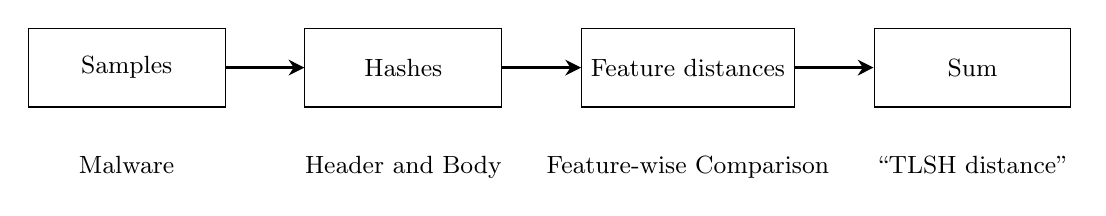
\begin{tikzpicture}[
				node distance=1cm,
				every node/.style={align=center, font=\small},
				process/.style={rectangle, draw, minimum width=2.5cm, minimum height=1cm},
				arrow/.style={-{Stealth[length=2mm, width=2mm]}, thick}
			]

			\node[process] (samples) {Samples};
			\node[process, right=of samples] (hash) {Hashes};
			\node[process, right=of hash] (comparison) {Feature distances};
			\node[process, right=of comparison] (distance) {Sum};

			\draw[arrow] (samples) -- (hash);
			\draw[arrow] (hash) -- (comparison);
			\draw[arrow] (comparison) -- (distance);

			\node[below=0.5cm of samples] {Malware};
			\node[below=0.5cm of hash] {Header and Body};
			\node[below=0.5cm of comparison] {Feature-wise Comparison};
			\node[below=0.5cm of distance] {\enquote{TLSH distance}};

		\end{tikzpicture}
	\end{adjustbox}
	\caption{TLSH File Comparison Pipeline}
	\label{fig:tlsh_pipeline}
\end{figure}

The formulae used to compute feature distances are specific to the features
being compared. For example, the formula for checksum (the first feature in
\autoref{fig:tlsh_structure}) distance can only output distances of zero or one.

Not mentioned in the whitepaper, but deeply relevant to this work, is
that most of these formulae are not metrics in the mathematical sense
because they do not all obey the triangle inequality. However, they are
semi-metrics because they are all symmetric, non-negative, and only yield
distances of zero when two features are the same.

The proofs of these claims are omitted for reasons of triviality: for example,
all TLSH formulae accumulate distance by either adding modular distances
(a counting-based distance metric \cite{oliverTLSHLocalitySensitive2013}),
positive constants, or absolute values of expressions
\cite{oliverTLSHLocalitySensitive2013}. As these all constitute
natural numbers, and as the naturals are closed under addition, TLSH distances
must also be naturals; and proof that TLSH distance violates the triangle
inequality follows trivially from the proof that TLSH can violate the triangle
inequality by 430 distance units, which I include in \ref{supplementals},
complete with constructive examples. Others have also made constructive
(if not maximal) proofs available \cite{baggettTLSHDistanceMetric2023}.

\subsubsection{TLSH for malware forensics}

TLSH possesses several extremely valuable attributes for malware
forensics and analysis: TLSH is open and permissively licensed
\cite{oliverGitHubTrendmicroTlsh2024}, so unlike proprietary LSH schemes, there
are no limitations or costs associated with its access or usage. TLSH
also performs well in comparative evaluations, where--relative to
other high-uptake, fully general LSH schemes--it is both accurate,
and robust against adversarial attacks
\cite{oliverDesigningElementsFuzzy2021}. Finally, as a corollary of
doing well amongst high-uptake LSH schemes, TLSH benefits from strong
network effects, having been adopted by platforms like VirusTotal.

These features are of unique and substantial value to analysts as
they facilitate the sharing and broader use of TLSH hashes. For
example, because VirusTotal adopted TLSH, analysts can conduct
TLSH-similarity queries on the entire VirusTotal corpus
\cite{virustotalAdvancedCorpusSearch2024}.

\subsubsection{TLSH limitation}

Unfortunately, a TLSH technical limitation disrupts the viability of
large-corpora TLSH nearest-neighbor queries. Indeed, \enquote{due to
performance reasons}, VirusTotal throttles TLSH queries to a rate of
15 per minute for paying users and prohibits their use entirely for
non-paying users. Moreover, VirusTotal's TLSH indexing and querying
algorithms are private, and a review of the literature found no
public alternatives. This leaves no straightforward way for those in
the industry to bear the cost of self-hosting a similar service. The
lack of such tooling necessarily constrains analysts' ability to use
TLSH with large malware datasets.

This limitation stems from the fact that TLSH is only a semi-metric,
not a metric: it violates the triangle inequality.

In a metric space, the triangle inequality suggests that if Alice and
Bob are close, and if Bob and Eve are close, then one can use their
closeness to bound the distance between Alice and Eve. If TLSH were a
metric, VP trees \cite{yianilosDataStructuresAlgorithms1993} could enable
efficient nearest-neighbor searches, because TLSH hashes could be laid out
in such a way that these bounds can direct a search, and, in turn, enable
pruning of large areas of the search space.

Because TLSH does not obey the triangle inequality, the use of metric-based
techniques for nearest-neighbor searches is limited. Analysts ostensibly
must either conduct \textit{exhaustive linear scans} of the entirety of
a dataset, every time that a query is conducted; or analysts must use
\textit{approximate nearest-neighbor search} and sacrifice precision,
recall, or both.

\subsection{Related Work}

\subsubsection{Research into TLSH scalability}\label{scalability}

The official TLSH documentation contradicts the claims of this paper,
noting that \enquote{TLSH is very fast at nearest-neighbor search
	at scale \textelp{} being a distance metric (as per the
	mathematical definition) and hence has logarithmic search times
\textelp{} and in particular [obeys] the triangle inequality}
\cite{oliverTLSHTechnicalOverview2021}. However, this is misleading,
as the authors now publicly acknowledge that
\enquote{the [TLSH] distance function does not obey the triangle inequality}
\cite{oliverTLSHDistanceMetric2024} and is only
\enquote{an approximate distance metric} \cite{oliverHACTFastSearch2020}.

Prior work to improve TLSH's scalability has had varying degrees of
applicability. For instance, Trend Micro Research documented one
improvement to \textit{the use} of TLSH for clustering, centered
around the parallelization of a clustering algorithm
\cite{aliScalableMalwareClustering2020}. While this can improve
throughput on a system in (at best) direct proportion to the amount
of available system parallelism, it does not solve the high
computational costs of TLSH queries themselves; rather, it just
allows that cost to be distributed across more CPU cores.

Other Trend Micro Research work presented two different acceleration
structures for TLSH nearest-neighbor search: a random forest and a VP
tree \cite{oliverFastClusteringHigh2021}. This work avoids the
former because it only gives approximate results, as noted in the prior work.
The latter, as was also noted, is a path toward an exact algorithm, making it
highly relevant. This work builds off their VP tree concept.

A careful reader may note that VP trees were previously
implied to be incompatible with non-metric distance functions. The
prior work attempts to address this based on the premise that
because TLSH is still \enquote{within a constant of a metric}
\cite{oliverHACTFastSearch2020}, and because \enquote{distance
functions that are within a constant [factor] of a metric} can still
be accelerated, a special VP tree can still work
\cite{oliverHACTFastSearch2020,oliverFastClusteringHigh2021} if it
considers additional nodes. The flaw with that work is in the
implementation: the authors assume that the constant factor is 20
\cite{oliverTlshTlshClusterPylib2021}, which is incorrect.
To be correct, the authors should have used $430$ (see
\autoref{tab:tlsh_violations}). Unfortunately, applying
this correction reduces the performance of their implementation to that
of unaccelerated, linear scanning (see \autoref{fig:comparison_1}).

\subsubsection{Non-TLSH alternatives}

Several mainstream LSH schemes, like ssdeep \cite{kornblumSsdeep2017}
and sdhash \cite{roussevDataFingerprintingSimilarity2010}, can be
used as TLSH alternatives; however, these fail to solve the
underlying scalability problem and, in comparative evaluations,
perform much worse than TLSH in terms of accuracy and resistance to
adversarial manipulation \cite{oliverTLSHLocalitySensitive2013,
	oliverUsingRandomizationAttack2014,
paganiPrecisionRecallUnderstanding2018, azabMiningMalwareDetect2014}.

Other LSH schemes map to proper metric spaces
\cite{guImprovedMethodLocality2013,oprisaLocalitysensitiveHashingOptimizations2014},
theoretically enabling efficient nearest-neighbor search. However,
these have not gained widespread adoption, limiting opportunities
for their use.

Within digital malware forensics specifically, several LSH schemes
exist as specialized algorithms, like PermHash for Chromium extensions
\cite{jaredwilsonPermhashNoCurls2023}, or peHash for PE files
\cite{wicherskiPeHashNovelApproach2009}. These
specializations can be highly constraining: peHash, for example, will
never identify relationships in code similarity between Mac, Windows,
and Linux payloads, as ELF files are not PE files, and neither are Mach-O files.

While many non-LSH techniques exist \cite{haqSurveyBinaryCode2021},
none were identified in the literature with the compactness
\cite{oliverTLSHLocalitySensitive2013}, throughput
\cite{oliverTLSHLocalitySensitive2013, haqSurveyBinaryCode2021,
liTopologyAwareHashingEffective2019}, generality
\cite{oliverTLSHLocalitySensitive2013}, and wide uptake of LSH schemes.

\section{Methods}\label{Methods}

This research is divided into three sections: theoretical
analysis to formalize TLSH's triangle inequality violations,
algorithm design to exploit the theoretical results, and comparison
of the devised algorithms to alternatives.

\subsection{Theory}

I first proved bounds on the degree to which TLSH subcomponents
could violate the triangle inequality, formalizing the proof using
the Lean v4.14.0 \cite{deMouraUllrich2021} proof-assistant and
mathematical library \cite{Mathlib}.

Specifically, letting $H_1, H_2, H_3$ be any three distinct TLSH
hashes, and letting $d(x, y)$ represent the contribution of a feature
of TLSH to the total TLSH distance, I solved for the tightest bounds
on $c$ in the triangle inequality, $d(H_1, H_3) \leq d(H_1, H_2) +
d(H_2, H_3) + c$.

Building on those results, I showed bounds for the TLSH distance
function and its constituent header and body components. For the
proof itself, see \ref{supplementals}.

\subsection{Algorithm Design}

I implemented and tested the following algorithms. For each,
\ref{Pseudocode} includes pseudocode.

\subsubsection{VP tree}

I implemented a VP tree
\cite{yianilosDataStructuresAlgorithms1993,uhlmannSatisfyingGeneralProximity1991},
inspired by prior work \cite{oliverHACTFastSearch2020}.

Unlike existing methods, this VP tree exclusively indexes the TLSH header
component, which, in theory, confers two advantages over indexing the
entirety of a TLSH hash: faster VP tree index construction because
body feature distance never needs to be computed; and faster VP tree
queries because header component distance violates the triangle
equality to a much lesser degree than body component distance, which
allows for more aggressive pruning during searches.

Because body component distance still matters, it is checked before a
candidate is added to the resulting nearest-neighbor list; if the sum
of header and body distance for two hashes is outside the
\enquote{cutoff} for what defines a nearby-neighbor, it is pruned.

\subsubsection{Trie with schema-learning}

I implemented a novel, trie-based \cite{fredkinTrieMemory1960}
approach to nearest-neighbor queries. Rather than search for nearby
neighbors in the order that TLSH features are laid out in a hash,
it uses a greedy, randomized algorithm to find an ordering, or
``schema,'' that maximizes the number of nodes pruned at shallow
levels of the search tree.

Trie search follows the ordering laid out in the schema. Helpfully,
schemas can be saved and reused on different datasets. In trie
search, the proofs of each TLSH feature's contributions to the total
triangle inequality violation are used to constrain the search radius.

\subsubsection{Replication of prior work}

I implemented and evaluated the VP tree design described by
Trend Micro Research \cite{oliverTlshTlshClusterPylib2021} in Rust
in order to evaluate performance relative to prior work.

Concerning the correctness issue outlined in Section \ref{scalability},
I tested ``corrected" and ``uncorrected" versions of their algorithm.

\subsubsection{Linear scanning}

Linear scanning served as a control.

Though largely outside the scope of the paper, the source code for
this work includes a parallel, Tensorflow-accelerated
\cite{martinabadiTensorFlowLargeScaleMachine2015} Python library for
working with TLSH on large datasets. \ref{Python} covers the
performance of its linear scanning routine.

\subsection{Empirical Evaluation}

\subsubsection{Datasets}
I evaluated performance on two datasets: randomly generated synthetic TLSH
hashes, and a convenience sample of 1,263,016 TLSH hashes sourced from the
VirusTotal metadata for a local repository of VirusShare
\cite{VirusSharecom2024} data.

The latter dataset represents the entirety of an employer-maintained
collection of data. Data was not filtered prior to or during the
evaluation. Furthermore, and in the interest of transparency, the
data is provided in the source code associated with the paper
(see \ref{supplementals}).

\subsubsection{Workloads}
This work examined three groups of nearest-neighbor search workloads,
based on common analytical tasks.

\enquote{Near} neighbors were defined as those with a TLSH distance
of at most 30, as this is a standard industry and academic choice
\cite{hutelmyerImplementingTLSHBased2024,joyceAVScan2VecFeatureLearning2023}
with TLSH. Larger cutoffs trade precision for recall
\cite{oliverTLSHLocalitySensitive2013}.

\begin{enumerate}
	\item All-to-all workloads:

		An analyst may receive a set of samples to triage and want to cluster them.

		To approximate inefficient clustering algorithms, I do pairwise
		comparisons of every sample in corpora of sizes 5,000 and 10,000.

	\item Fixed-query-size, variable-corpora-size workloads:

		An analyst may receive a set of samples to triage and want to check
		which are novel.

		To approximate this task, I measured the time it took to conduct
		1,000 queries on various-sized subsets of a larger corpus. The
		queries were chosen randomly from the larger corpus rather than its subset.

	\item Variable-query-size, variable-corpora-size workloads:

		An analyst may use TLSH and a specialized clustering algorithm
		requiring very few comparisons.

		To approximate more efficient clustering algorithms, I measured
		the time it took to query a random 10\% of corpora of various
		sizes. The sampling procedure is the same as for the
		fixed-query-size, variable-corpora-size workload.

\end{enumerate}

To assess whether the choice of $30$ as a
distance cutoff biased the results and to capture alternative
workloads, I evaluated cutoffs from 1 to 1,000. Note
that at cutoffs above 200, TLSH may exceed a false-positive rate of 50\%
\cite{oliverTLSHLocalitySensitive2013}, so measurements past that
point are of questionable utility.

To assess whether aspects of these workloads were \enquote{shifted}
from query-time to preprocessing-time in a way that might prove too
computationally demanding or wasteful for specific tasks, I also
evaluated the time spent building the acceleration structures.

Note that because a single schema may be reused with different
corpora, the choice to do schema-learning (rather than reuse a
single schema) represents a trade-off between data structure
efficiency and preprocessing time. Although this has little influence
on results, I show measurements of trie preprocessing with and
without schema-learning.

\subsubsection{Benchmark environment}

I ran all benchmarks 11 times on a 12-core M2 Max MacBook Pro using
high-performance mode on macOS 15.2. Reported results represent
median execution times. The testing harness and associated algorithms
were built with Rust 1.83.0. The benchmark suite recorded CPU clock
speeds using the sysinfo crate \cite{SysinfoCratesioRust2024}.
The records showed no indications of throttling.

\section{Results}

\subsection{Theory}
I quantified the contribution of different TLSH features to the
total violation of the triangle inequality.
For information regarding the proof, please see \ref{supplementals}.

\vspace*{-0.5\baselineskip}

\begin{table}[H]
	\centering
	\begin{tabular}{|l|c|}
		\hline
		\textbf{Component}                       & \textbf{Violation} \\ \hline
		\multicolumn{2}{|c|}{\textbf{Header Distance Violations}}     \\ \hline
		Checksum-distance                        & 0                  \\ \hline
		L-distance                               & 22                 \\ \hline
		q$_1$-distance                           & 12                 \\ \hline
		q$_2$-distance                           & 12                 \\ \hline
		\textbf{Total Header Distance}           & \textbf{46}        \\ \hline
		\multicolumn{2}{|c|}{\textbf{Body Distance Violations}}       \\ \hline
		Per-bucket body distance                 & 3                  \\ \hline
		\textbf{Total Body Distance} (128 buckets) & \textbf{384}     \\ \hline
		\textbf{Overall Violation}               & \textbf{430}       \\ \hline
	\end{tabular}
	\caption{TLSH triangle inequality distance violations}
	\label{tab:tlsh_violations}
\end{table}

\vspace*{-1.5\baselineskip}

\subsection{Scaling by Workload and Data Source}
\autoref{fig:comparison_1} shows algorithm performance when the
cutoff for similarity is 30 and corpora sizes are varied.
\autoref{fig:comparison_2} shows the performance of the algorithms
when only the cutoff for similarity is varied.

\clearpage

\begin{figure*}
	\centering

	\begin{subfigure}[b]{0.97\columnwidth}
		\centering
		\includegraphics[width=\textwidth]{\plotspath/line_plots/random/query_time_fixed/query_time_fixed_logy.pdf}
		\caption{Relationship between corpus size
			and time to query 1,000
		hashes in randomly generated hash corpora.}
		\label{fig:random_corpus_vs_total_time}
	\end{subfigure}
	\hfill
	\begin{subfigure}[b]{0.97\columnwidth}
		\centering
		\includegraphics[width=\textwidth]{\plotspath/line_plots/file/query_time_fixed/query_time_fixed_logy.pdf}
		\caption{Relationship between corpus size
			and time to query 1,000
		hashes in VirusShare-derived hash corpora.}
		\label{fig:file_corpus_vs_total_time}
	\end{subfigure}
	\vspace{1em}

	\begin{subfigure}[b]{0.97\columnwidth}
		\centering
		\includegraphics[width=\textwidth]{\plotspath/line_plots/random/time_to_query_10_percent/time_to_query_10_percent_logy.pdf}
		\caption{Relationship between corpus size
			and total build and
		query time, when querying 10\% of randomly generated hash corpora.}
		\label{fig:random_corpus_vs_query_time}
	\end{subfigure}
	\hfill
	\begin{subfigure}[b]{0.97\columnwidth}
		\centering
		\includegraphics[width=\textwidth]{\plotspath/line_plots/file/time_to_query_10_percent/time_to_query_10_percent_logy.pdf}
		\caption{Relationship between corpus size
			and total build and
		query time, when querying 10\% of VirusShare-derived hash corpora.}
		\label{fig:file_corpus_vs_query_time}
	\end{subfigure}

	\vspace{1em}

	\begin{subfigure}[b]{0.97\columnwidth}
		\centering
		\includegraphics[width=\textwidth]{\plotspath/line_plots/random/average_build_and_schema_time/average_build_and_schema_time_logy.pdf}
		\caption{Relationship between corpus size and index build time for
		randomly generated hashes.}
		\label{fig:build_time_random}
	\end{subfigure}
	\hfill
	\begin{subfigure}[b]{0.97\columnwidth}
		\centering
		\includegraphics[width=\textwidth]{\plotspath/line_plots/file/average_build_and_schema_time/average_build_and_schema_time_logy.pdf}
		\caption{Relationship between corpus size and index build time for
		VirusShare-derived hashes.}
		\label{fig:build_time_file}
	\end{subfigure}

	\vspace{1em}

	\caption{Assorted performance metrics for the various algorithms
	with cutoff of 30.}
	\label{fig:comparison_1}
\end{figure*}

\clearpage

\begin{figure*}
	\centering

	\begin{subfigure}[b]{0.97\columnwidth}
		\centering
		\includegraphics[width=\textwidth]{\plotspath/line_plots/random/total_time_vs_cutoff/query_time_vs_cutoff_logy.pdf}
		\caption{Relationship between cutoff and
			time to query 1,000 of
		1,000,000 random hashes.}
		\label{fig:random_cutoff_vs_query_time}
	\end{subfigure}
	\hfill
	\begin{subfigure}[b]{0.97\columnwidth}
		\centering
		\includegraphics[width=\textwidth]{\plotspath/line_plots/file/total_time_vs_cutoff/query_time_vs_cutoff_logy.pdf}
		\caption{Relationship between cutoff and
			time to query 1,000 of
		1,000,000 VirusShare-derived hashes.}
		\label{fig:file_cutoff_vs_query_time}
	\end{subfigure}
	\hfill

	\vspace{1em}

	\begin{subfigure}[b]{0.97\columnwidth}
		\centering
		\includegraphics[width=\textwidth]{\plotspath/line_plots/random/total_time_vs_cutoff/total_time_vs_cutoff_logy.pdf}
		\caption{Relationship between cutoff and
			total build and query time
		for 1,000 queries of 1,000,000 random hashes.}
		\label{fig:random_cutoff_vs_total_time}
	\end{subfigure}
	\hfill
	\begin{subfigure}[b]{0.97\columnwidth}
		\centering
		\includegraphics[width=\textwidth]{\plotspath/line_plots/file/total_time_vs_cutoff/total_time_vs_cutoff_logy.pdf}
		\caption{Relationship between cutoff and
			total build and query time
		for 1,000 queries of 1,000,000 VirusShare-derived hashes.}
		\label{fig:file_cutoff_vs_total_time}
	\end{subfigure}

	\vspace{1em}

	\begin{subfigure}[b]{0.97\columnwidth}
		\centering
		\includegraphics[width=\textwidth]{\plotspath/line_plots/random/build_and_schema_time_vs_cutoff/build_and_schema_time_vs_cutoff_logy.pdf}
		\caption{Relationship between cutoff and
		build time (with and without schema-learning) for 1,000,000 random hashes.}
		\label{fig:random_cutoff_vs_build_time}
	\end{subfigure}
	\hfill
	\begin{subfigure}[b]{0.97\columnwidth}
		\centering
		\includegraphics[width=\textwidth]{\plotspath/line_plots/file/build_and_schema_time_vs_cutoff/build_and_schema_time_vs_cutoff_logy.pdf}
		\caption{Relationship between cutoff and
			build time (with and without schema-learning) for 1,000,000
		VirusShare-derived hashes.}
		\label{fig:file_cutoff_vs_build_time}
	\end{subfigure}

	\vspace{1em}

	\caption{Effect of different cutoff levels on algorithm performance.}
	\label{fig:comparison_2}
\end{figure*}

\clearpage

\subsection{Fixed-Workload Results}
Both indices outperformed linear scanning on the 10,000-to-10,000,
cutoff-of-30, clustering-like workloads. The VP tree was strictly
faster than the trie on real-world data.

\begin{figure}[H]
	\centering
	\includegraphics[width=\columnwidth]{\plotspath/consolidated_bar_charts/corpus_10000/query_10000/cutoff_30/consolidated/consolidated_bar_chart_query10000_corpus10000.pdf}
	\caption{Median profile of an all-to-all workload involving a
	10,000-hash corpus, by data source.}
	\label{fig:all_to_all_bar_chart}
\end{figure}

Results were similar on 1,000-to-1,000,000 workloads.

\begin{figure}[H]
	\centering
	\includegraphics[width=\columnwidth]{\plotspath/consolidated_bar_charts/corpus_1000000/query_1000/cutoff_30/consolidated/consolidated_bar_chart_query1000_corpus1000000.pdf}
	\caption{Median profile of a 1,000-to-1,000,000 workload,
	by data source.}
	\label{fig:1k_to_1m_chart}
\end{figure}

\section{Discussion}

The results make for several substantial contributions to the TLSH
scalability literature.

The analysis of TLSH's triangle inequality violations was the most
relevant to prior literature because it demonstrated errors in prior
work. \autoref{tab:tlsh_violations} showed that the triangle
inequality could be violated by a constant factor of 430, far
exceeding the prior estimate of 20
\cite{oliverTlshTlshClusterPylib2021}. After correcting this error in
the prior work, its performance degraded to that of linear scanning
(see \autoref{fig:file_corpus_vs_total_time}).

The results on synthetic data were much better for the acceleration
structures than the results on real-world data. This discrepancy
likely stems from the tighter distribution of TLSH features in
real-world data. For example, file length--a key TLSH feature--has
much lower variance in real-world datasets than in randomly
generated data. This tighter clustering means hashes have more
plausibly nearby neighbors, reducing opportunities for pruning during
queries. This analysis focuses on real-world data to avoid drawing
biased conclusions.

\subsection{VP Tree}

Compared to the corrected prior work and linear scanning, I see much
better performance--over an order of magnitude greater throughput at the
standard cutoff of 30--with the presented VP tree. The uplift was in both
index construction (\autoref{fig:build_time_file}) and querying
(\autoref{fig:file_corpus_vs_query_time}), due to reduced
computational overhead during construction (as body distance does not
get used) and more aggressive pruning during searches, respectively.

The VP tree demonstrated performance advantages during index
construction at all cutoff levels and against all tested data
structures (see \autoref{fig:file_cutoff_vs_build_time}).

Although the VP tree underperformed linear scanning at extremely wide
similarity cutoffs, at every cutoff below 200--when $\geq\!50\%$
false positive rates are known to occur
\cite{oliverTLSHLocalitySensitive2013} and broader cutoffs are likely
to be impractical--the VP tree was the fastest technique
(see \autoref{fig:file_cutoff_vs_total_time}).

The advantage was particularly pronounced in
\autoref{fig:file_cutoff_vs_query_time}, which represents cases where
index construction times amortize away; here, the VP tree was
the best performing up to cutoffs of approximately 400.

\subsection{Trie}

I diverged from prior work by introducing a novel,
trie-based VP tree alternative for TLSH nearest-neighbor search. At
very strict cutoffs, the trie outperforms the VP tree and
the prior work by an order of magnitude, but this advantage quickly
vanishes at higher cutoff values. At cutoffs above 10, the VP tree
shows a consistent performance advantage, and at cutoffs above 100,
the trie underperforms linear scanning. This stark regression is
likely because, with each query, the trie performs an exhaustive
breadth-first search. It is only because of aggressive pruning,
which requires tight cutoffs, that trie search is performant.

\subsection{Linear scanning}

Because linear scanning performance is unaffected by cutoff (see
\autoref{fig:file_cutoff_vs_total_time}), linear scanning may be
advantageous in certain ultra-high-cutoff use cases. On smaller
corpora, even when linear scanning is slower than querying indexed
structures, highly demanding workloads like all-to-all queries can
still be completed in seconds (see
\autoref{fig:all_to_all_bar_chart}). Consequently, there may be cases
where linear scanning is preferable to indexed searches for speed or
convenience.

Nevertheless, linear scanning performance degrades quickly with
larger corpora and more queries. \autoref{fig:1k_to_1m_chart}
demonstrates this limitation, showing a large performance gap between
the index-based algorithms and linear scanning.

\subsection{Implications}

The results were highly pronounced on clustering workloads, where the
best algorithm--the VP tree--delivered a $10\times$ performance uplift
compared to the state-of-the-art
(see \autoref{fig:file_corpus_vs_total_time}).
Though difficult to see on a log scale, performance \textit{scaling}
was also much better with the VP tree than with the prior work.

Unlike clustering workloads, where the number of nearest-neighbor
queries grows with the size of the dataset, malware corpus search
APIs like VirusTotal's \enquote{Advanced Corpus Search}
\cite{virustotalAdvancedCorpusSearch2024} represent workloads that
consist entirely of a single nearest-neighbor query. For these APIs
and workloads, performance improvements for queries directly
translate to increased API or analyst capacity: at a cutoff of 30,
compared to the prior state-of-the-art, a nearest-neighbor search API
using the VP tree can either dispatch ten times as many queries or
query a dataset ten times the size, with the same compute budget.

\section{Conclusion}

I used a formal proof assistant to demonstrate fundamental
limitations in TLSH and in prior TLSH nearest-neighbor search
implementations. I then leveraged the formal results to design two
data structures that could overcome these limitations: one based on
a vantage-point tree, and another based on a trie-like structure.

I found that on real-world data, for nearest-neighbor querying tasks
and associated clustering workloads, these algorithms provided one to
two orders of magnitude greater throughput relative to the state of
the art. Except at the most stringent cutoffs for what constitutes a
``near neighbor,'' the VP tree was the fastest of the two data
structures. Accordingly, this performance improvement allows
analysts to process datasets an order of magnitude larger than what
was previously feasible with the same resources.

\section{Acknowledgments}

I want to acknowledge Corvus Forensics for maintaining the VirusShare
dataset, which made it viable to test on real-world data. I would
also like to thank MITRE and MITRE's sponsors for sponsoring this
research, particularly Brian Shaw, Christopher Andersen,
Dan Perret, Dr. Justin Brunelle, Frank Posluszny, Laurence Hunter,
Morgan Keiser, and Tim McNevin.

I want to give additional thanks to Brian Shaw,
Christopher Andersen, Dr. Justin Brunelle, and Tim McNevin for their
invaluable constructive criticism; Frank Posluszny, for his feedback and
for providing me with the malware metadata from which the real-world
TLSH digests were extracted; and Laurence Hunter, for his mentorship,
generosity, and feedback, without which this could not have been written.

This software (or technical data) was produced for the
U.S.~Government and is subject to the Rights in Data-General Clause
52.227-14, Alt.~IV (May 2014) -- Alternative IV (Dec 2007).

\bibliographystyle{elsarticle-num}
\bibliography{paper-dependencies/latex-dependencies/bibliography.bib}

\clearpage

\appendix

\section{Supplemental Material}\label{supplementals}

All supplemental material can be found at \supplementalsurl.

\section{Pseudocode}\label{Pseudocode}

All algorithms take in a data structure holding a corpus, a query, and a
radius used as the cutoff for similarity search.

The VP tree is constructed as any other: assume every node in the
tree is a vantage-point with radius of size \texttt{node.threshold}.
Little improvement was observed with different vantage-point selection
strategies. The approach described as ``prior literature" differs
only in $430$ being used as \texttt{MAX_HEADER_VIOLATION}, and with
the total distance being used instead of header distance.

\begin{algorithm}[H]
	\caption{Query logic for VP tree}
	\begin{algorithmic}
		\Function{range_query}{\texttt{tree}, \texttt{query}, \texttt{radius}}
		\State \texttt{results} $\gets$ [ ]
		\State \texttt{stack} $\gets$ [\texttt{tree.root}]
		\State \texttt{new\_radius} $\gets$ \texttt{radius} +
		\texttt{MAX\_HEADER\_VIOLATION}
		\While{\texttt{stack} not empty}
		\State \texttt{node} $\gets$ \texttt{stack.pop()}
		\State \texttt{header\_dist} $\gets$
		\Call{header_dist}{\texttt{node.point}, \texttt{query}}
		\State \texttt{body\_dist} $\gets$
		\Call{body_dist}{\texttt{node.point}, \texttt{query}}
		\If{\texttt{header\_dist} + \texttt{body\_dist} $\leq$ \texttt{radius}}
		\State append \texttt{node.point} to \texttt{results}
		\EndIf
		\If{\texttt{header\_dist} - \texttt{new\_radius} $\leq$
		\texttt{node.threshold}}
		\State append \texttt{node.left} to \texttt{stack}
		\EndIf
		\If{\texttt{header\_dist} + \texttt{new\_radius} $\geq$
		\texttt{node.threshold}}
		\State append \texttt{node.right} to \texttt{stack}
		\EndIf
		\EndWhile
		\State \Return \texttt{results}
		\EndFunction
	\end{algorithmic}
\end{algorithm}

The trie has both a searching component and a schema-learning component.

\begin{algorithm}[H]
	\caption{Trie schema-learning logic}
	\begin{algorithmic}

		\Function{learn_schema}{\texttt{data}, \texttt{cutoff}}
		\State \texttt{sample\_n} $\gets$ \Call{min}{64, $|$\texttt{data}$|$}
		\State \texttt{sampled\_data} $\gets$ randomly sample
		\texttt{sample\_n} from \texttt{data}
		\State \texttt{schema} $\gets$ [ ]
		\State \texttt{max\_cutoffs} $\gets$ $0$

		\Loop
		\State \texttt{best\_feature} $\gets$ \texttt{null}
		\State \texttt{best\_num_cutoffs} $\gets$ \texttt{max\_cutoffs}
		\State \texttt{best\_feature\_by\_sum} $\gets$ null
		\State \texttt{best\_sum} $\gets$ $0$

		\State \texttt{feature\_range} $\gets$ 0..36 \Comment{36 =
		\# TLSH features}

		\For{each \texttt{i} in \texttt{feature\_range}}
		\If{\texttt{schema} contains \texttt{i}}
		\State \textbf{continue}
		\EndIf

		\State \texttt{trial} $\gets$ \texttt{schema} + [\texttt{i}]

		\State \texttt{num\_cutoffs} $\gets$ 0
		\State \texttt{total\_sum} $\gets$ 0

		\For{each \texttt{v} in \texttt{sampled\_data}}
		\State \texttt{pair\_cutoffs} $\gets$ 0
		\State \texttt{pair\_sum} $\gets$ 0
		\For{each \texttt{u} in \texttt{sampled\_data}}
		\State \texttt{diff} $\gets$ \Call{feature_dist}{\texttt{u},
		\texttt{v}, \texttt{trial}}
		\If{\texttt{diff} $\geq$ \texttt{cutoff}}
		\State \texttt{pair\_cutoffs} $\gets$ \texttt{pair\_cutoffs + 1}
		\EndIf
		\State \texttt{pair\_sum} $\gets$ \texttt{pair\_sum} + \texttt{diff}
		\EndFor
		\State \texttt{num\_cutoffs} $\gets$ \texttt{num\_cutoffs} +
		\texttt{pair\_cutoffs}
		\State \texttt{total\_sum} $\gets$ \texttt{total\_sum} + \texttt{pair\_sum}
		\EndFor

		\If{\texttt{total\_sum} > \texttt{best\_sum}}
		\State \texttt{best\_sum} $\gets$ \texttt{total\_sum}
		\State \texttt{best\_feature\_by\_sum} $\gets$ \texttt{i}
		\EndIf

		\If{\texttt{num\_cutoffs} > \texttt{best\_num_cutoffs}}
		\State \texttt{best\_num_cutoffs} $\gets$ \texttt{num\_cutoffs}
		\State \texttt{best\_feature} $\gets$ \texttt{i}
		\EndIf
		\EndFor

		\If{\texttt{best\_feature} not \texttt{null}}
		\State append \texttt{best\_feature} to \texttt{schema}
		\ElsIf{\texttt{best\_feature\_by\_sum} not \texttt{null}}
		\State append \texttt{best\_feature\_by\_sum} to \texttt{schema}
		\Else
		\State \textbf{break}
		\EndIf

		\State \texttt{max\_cutoffs} $\gets$ \texttt{best\_num_cutoffs}
		\EndLoop
		\State \Return schema
		\EndFunction
	\end{algorithmic}
\end{algorithm}

\begin{algorithm}[H]
	\caption{Trie query logic}
	\begin{algorithmic}

		\Function{trie_search}{\texttt{node}, \texttt{query},
		\texttt{radius}, \texttt{schema}}
		\If{\texttt{node} is a leaf}
		\State \Return \Call{Filter}{\texttt{node.points},
		\texttt{query}, \texttt{radius}, \texttt{schema}} \Comment{Filter
		out would-be false-positives using remaining features}
		\EndIf
		\State \texttt{results} $\gets$ [ ]
		\State \texttt{feature} $\gets$ first feature in \texttt{schema}
		\State \texttt{value} $\gets$
		\Call{get_feature_value}{\texttt{query}, \texttt{feature}}
		\State \texttt{max\_diff} $\gets$
		\Call{compute_max_diff}{\texttt{feature}, \texttt{radius}}
		\For{all possible \texttt{candidate} value s.t.
		\texttt{candidate} diff $\in$ $[0, \texttt{max\_diff}]$}
		\Comment{\texttt{diff} > \texttt{max\_diff} $\to$ \texttt{dist} >
		\texttt{radius}}
		\State \texttt{dist} $\gets$ \Call{feature_diff}{\texttt{value},
		\texttt{candidate}, \texttt{feature}}
		\If{\texttt{dist} $\leq$ \texttt{radius}}
		\State \texttt{child} $\gets$ \texttt{node}[\texttt{candidate}]
		\State \texttt{radius\_budget} $\gets$ \texttt{radius} - \texttt{dist}
		\State \texttt{schema'} $\gets$ \Call{tail}{schema}
		\State \texttt{sub\_results} $\gets$
		\Call{trie_search}{\texttt{child}, \texttt{query},
		\texttt{radius\_budget}, \texttt{schema'}}
		\For{each \texttt{sub_result} in \texttt{sub_results}}
		append \texttt{sub\_result} to \texttt{results}
		\EndFor
		\EndIf
		\EndFor
		\State \Return \texttt{results}
		\EndFunction
	\end{algorithmic}
\end{algorithm}

For completeness, \texttt{linear_scan} is as follows:
\begin{algorithm}[H]
	\caption{Linear scan}
	\begin{algorithmic}
		\Function{linear_scan}{\texttt{corpus}, \texttt{query}, \texttt{radius}}
		\State \texttt{results} $\gets$ [ ]
		\For{\texttt{digest} in \texttt{corpus}}
		\State \texttt{header\_dist} $\gets$
		\Call{header_dist}{\texttt{digest}, \texttt{query}}
		\State \texttt{body\_dist} $\gets$
		\Call{body_dist}{\texttt{digest}, \texttt{query}}
		\If{\texttt{header\_dist} + \texttt{body\_dist} $\leq$ \texttt{radius}}
		\State append \texttt{digest} to \texttt{results}
		\EndIf
		\EndFor
		\State \Return \texttt{results}
		\EndFunction
	\end{algorithmic}
\end{algorithm}

\section{Tensorflow-accelerated scanner}\label{Python}

I authored a Tensorflow-accelerated linear scanning routine to
facilitate using TLSH on large datasets, within Python notebooks. I
benchmarked it against a linear scanning routine powered by py-tlsh
\cite{PytlshTLSHPython2024}, the official \cpluspluslogo\, Python
extension for fast TLSH operations.

The benchmarks used Rust 1.83.0, Python 3.12.7, Tensorflow 2.18.0
\cite{martinabadiTensorFlowLargeScaleMachine2015}, numpy 2.0.1
\cite{harris2020array}, and py-tlsh 4.7.2 \cite{PytlshTLSHPython2024}.

I included Rust linear scanner performance for illustrative purposes
only, as the Rust and Python benchmark harnesses differ, limiting
result comparability.

The benchmark results were as follows:

\begin{figure}[H]
	\centering
	\includegraphics[width=\columnwidth]{\plotspath/python_comparative_chart.pdf}
	\caption{Performance of linear-scan implementations.}
	\label{fig:python_linear_scan}
\end{figure}

The Tensorflow-enhanced Python library outperformed the py-tlsh-based scanner
across all measured workloads.

I attribute a roughly 10x
performance uplift, relative to the py-tlsh-based scanner, to
parallelism; and the residual performance uplifts to two factors:
that Tensorflow
optimizes memory access patterns, particularly on all-to-all tasks;
and that Tensorflow batches queries, which reduces the time spent in the Python
interpreter.

The benchmark code is available in \ref{supplementals}.

\end{document}
